\section{Additional Stability Ablations}
\label{sec:stability-ablations}

We include all training curves for our hyperparameter sweep experiments in \cref{sec:hyperparameters}. We conduct a learning rate sweep over $\{ 2e-4, 4e-4, 6e-4, 8e-4, 1e-3\}$ observing that Parcae exhibits stable training over both baseline Pre-Norm RDMs and residual normalized RDMs. The training curves and the accompanying recurrent state norm can be observed in \cref{fig:all-instability-curves}.

\begin{figure}
    \centering
    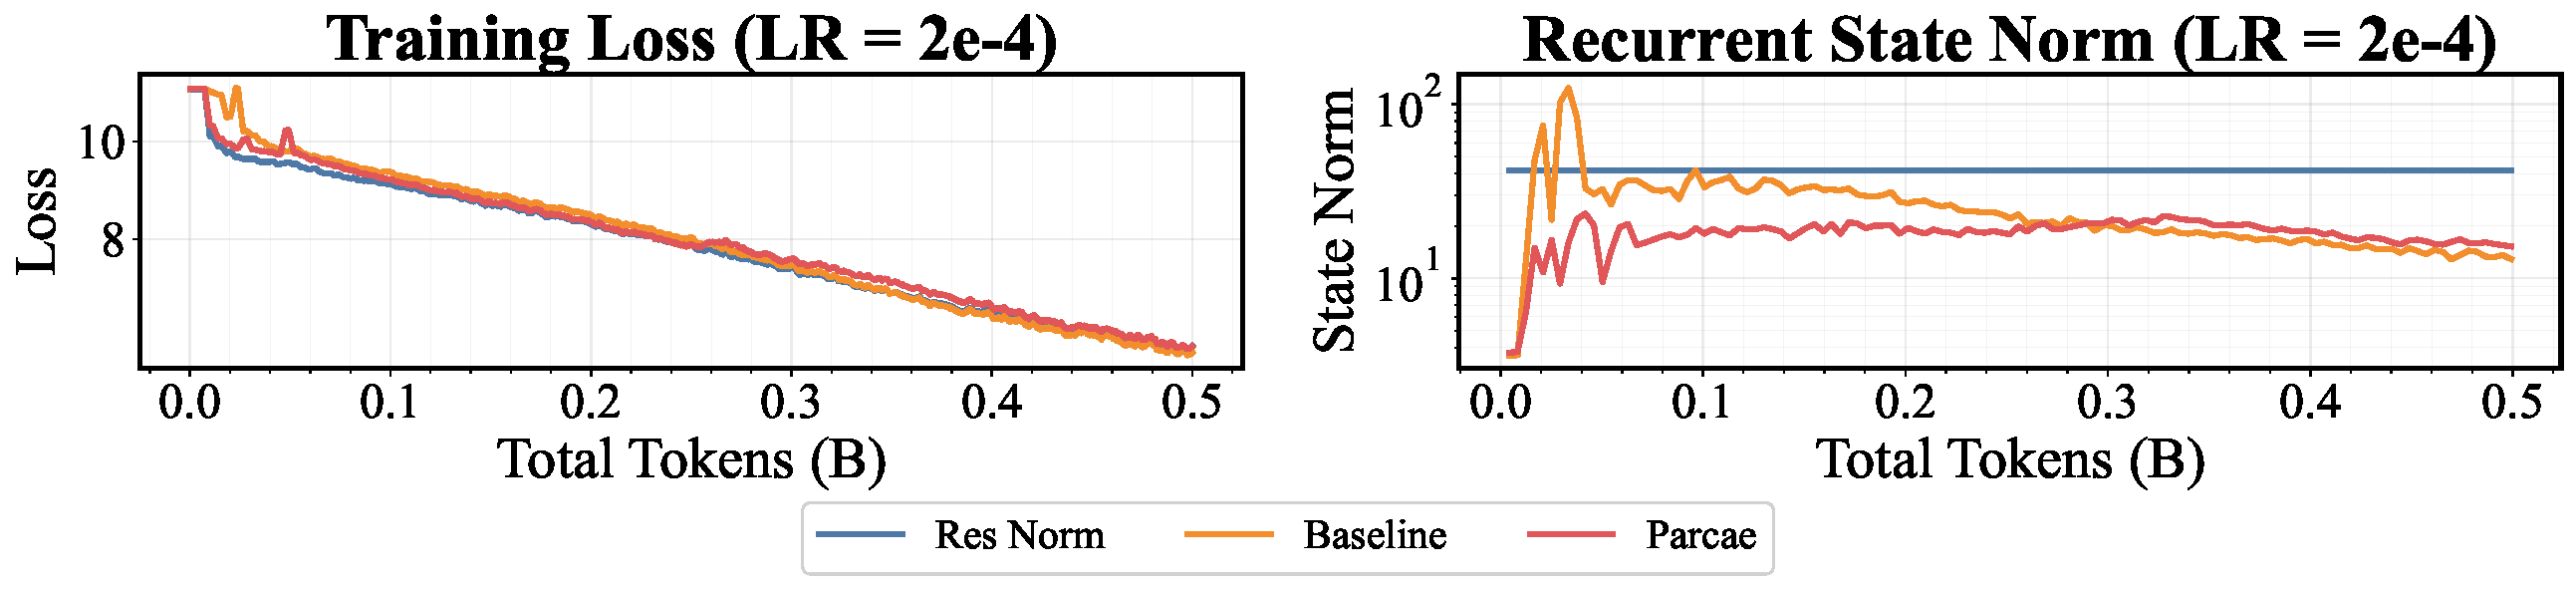
\includegraphics[width=\linewidth]{figures/appendix/instability/instability_lr_2e-4.pdf}
    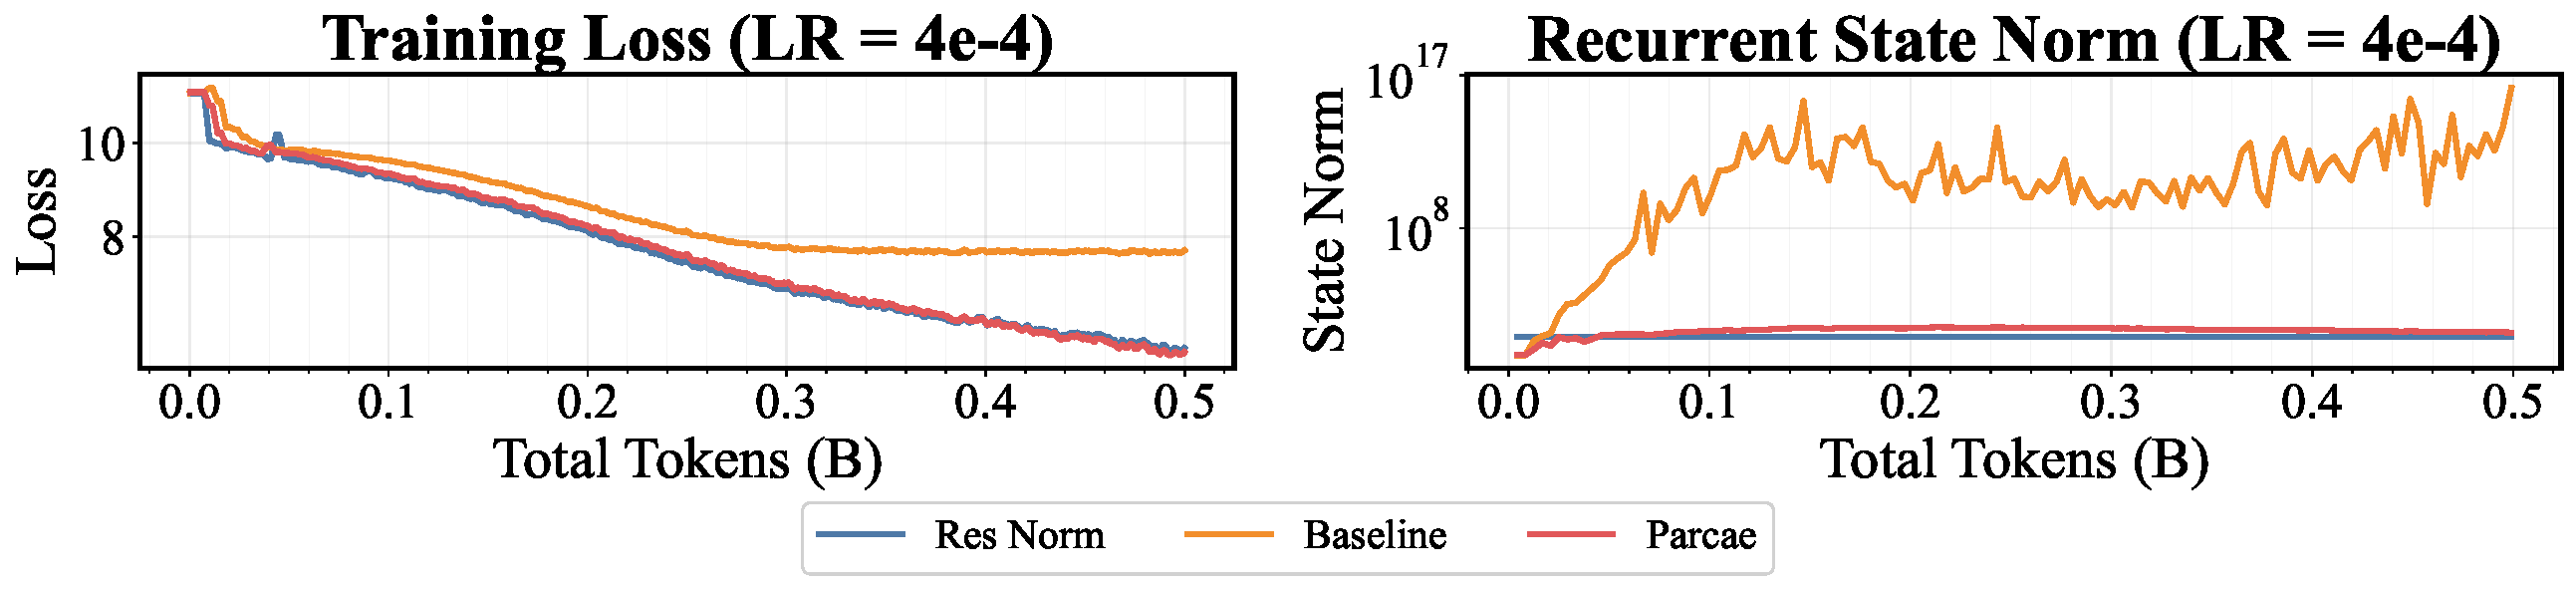
\includegraphics[width=\linewidth]{figures/appendix/instability/instability_lr_4e-4.pdf}
    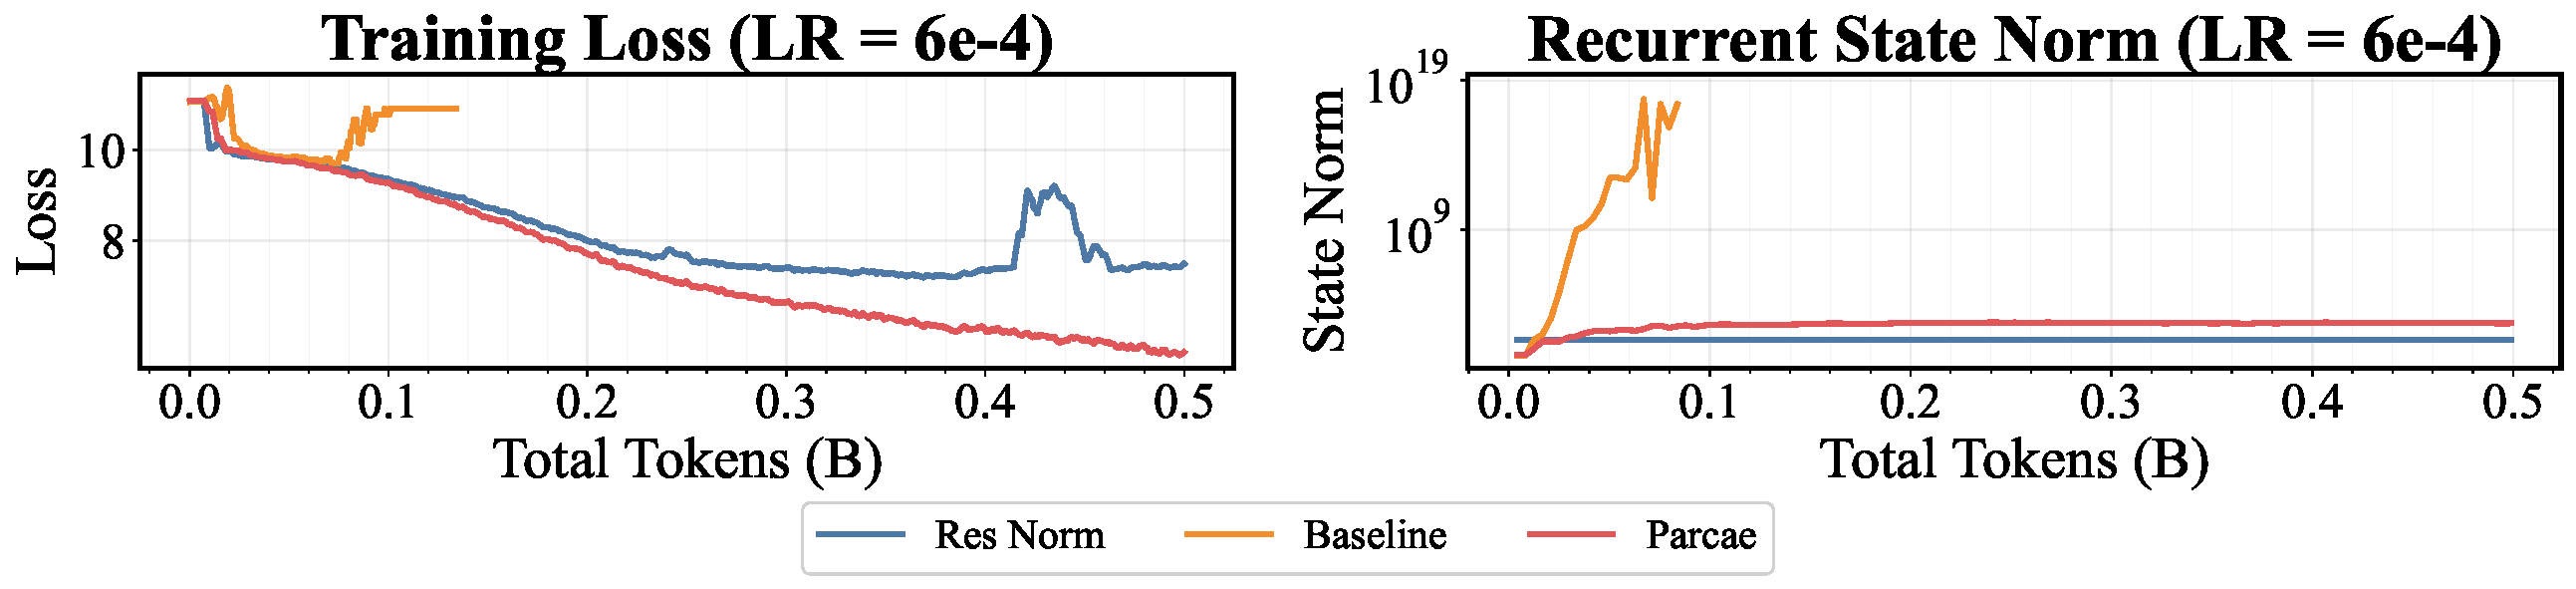
\includegraphics[width=\linewidth]{figures/appendix/instability/instability_lr_6e-4.pdf}
    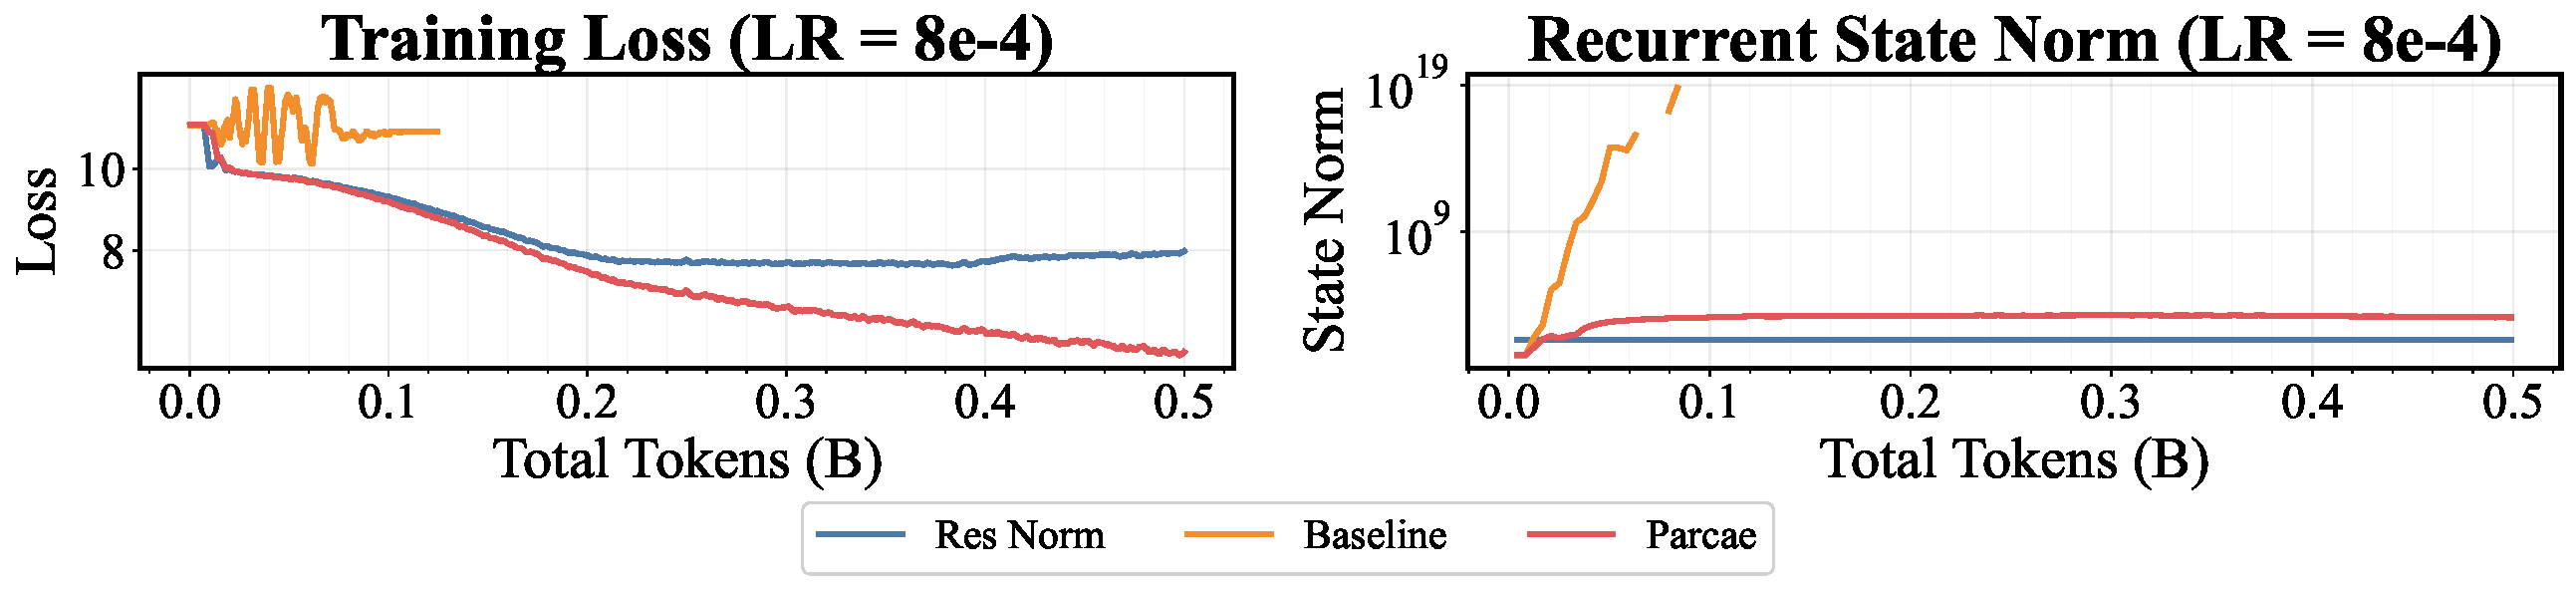
\includegraphics[width=\linewidth]{figures/appendix/instability/instability_lr_8e-4.pdf}
    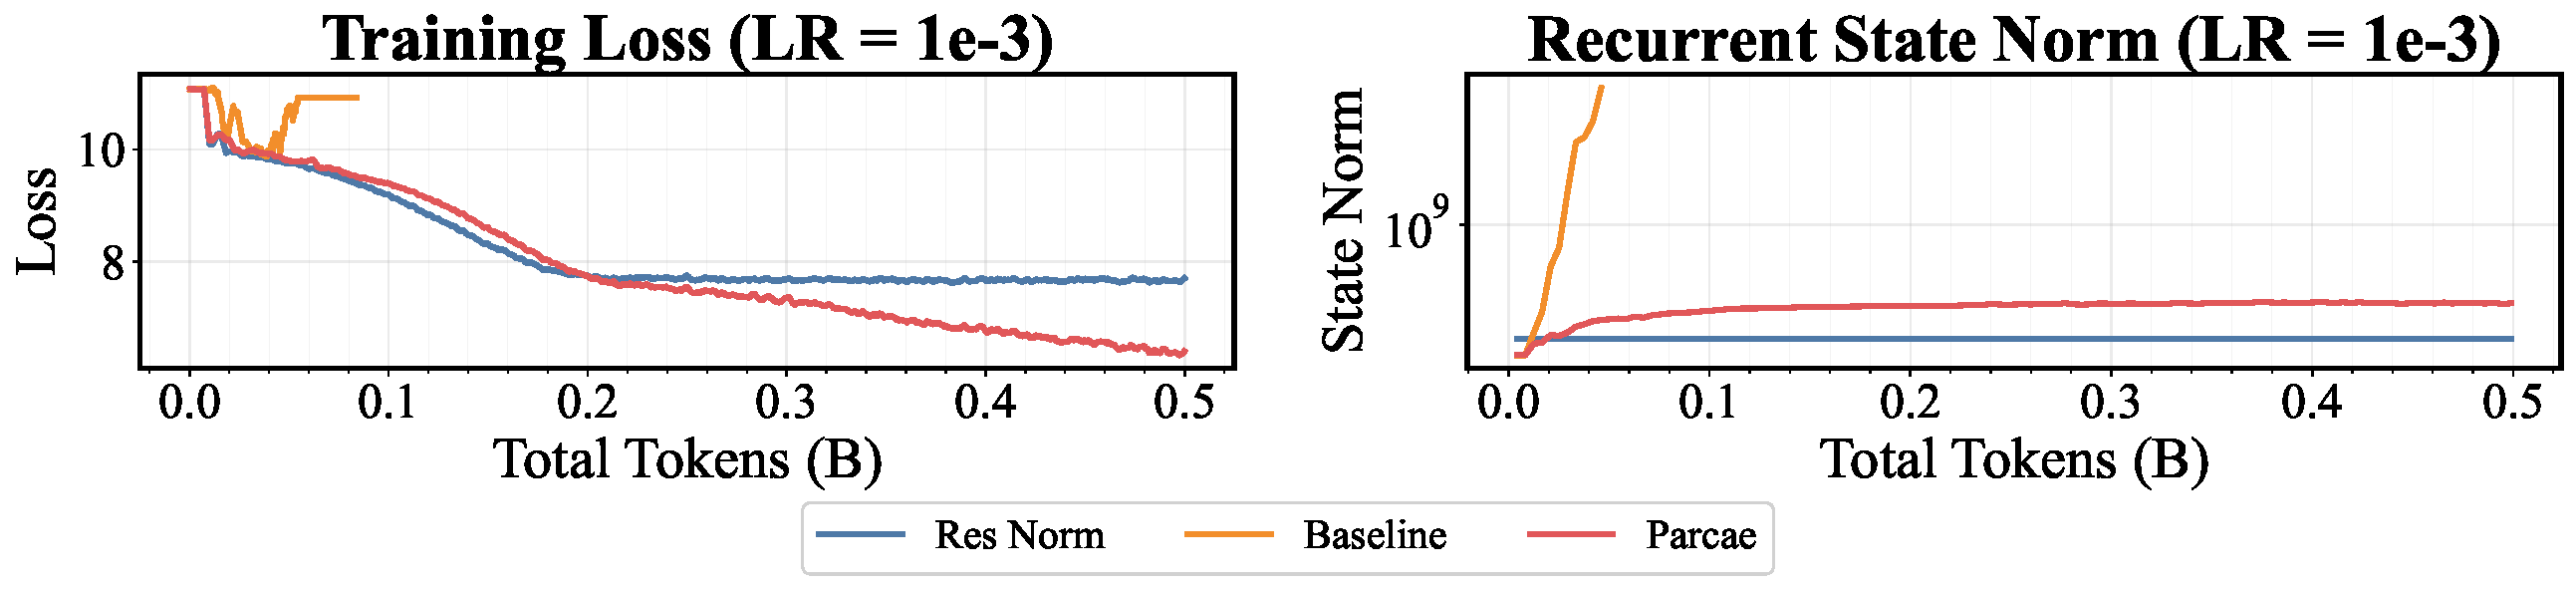
\includegraphics[width=\linewidth]{figures/appendix/instability/instability_lr_1e-3.pdf}
    \caption{Training instability of recurrent depth models across different learning rates. We show both training losses and recurrent state norm to understand divergence and state explosion.}
    \label{fig:all-instability-curves}
\end{figure}
